\tableofcontents

\section{Definitions}
Trough this manual we will assume that the system is installed and properly working, and that the domain where this system is installed is \verb|example.com|
To use the system, you need to open a browser compatible with html5, like Google chrome, Safari, Microsoft Internet Explorer 10+, Microsoft Edge or Mozilla Firefox, we've not tested on Opera, but it might work too.

\section{Login}
Proceed to the site url by opening the browser and at the address bar type: www.example.com[/install/path]\footnote{/install/path is optional and must be replaced by the installation path on the server, from the public\_html folder, relative, not absolute, so if the system is installed in ~/public\_html/checker, the url will be www.example.com/checker}
You will be presented with the following screen:

\begin{figure*}[ht!]
	\caption{Login screenshot}
	\label{img:login}
	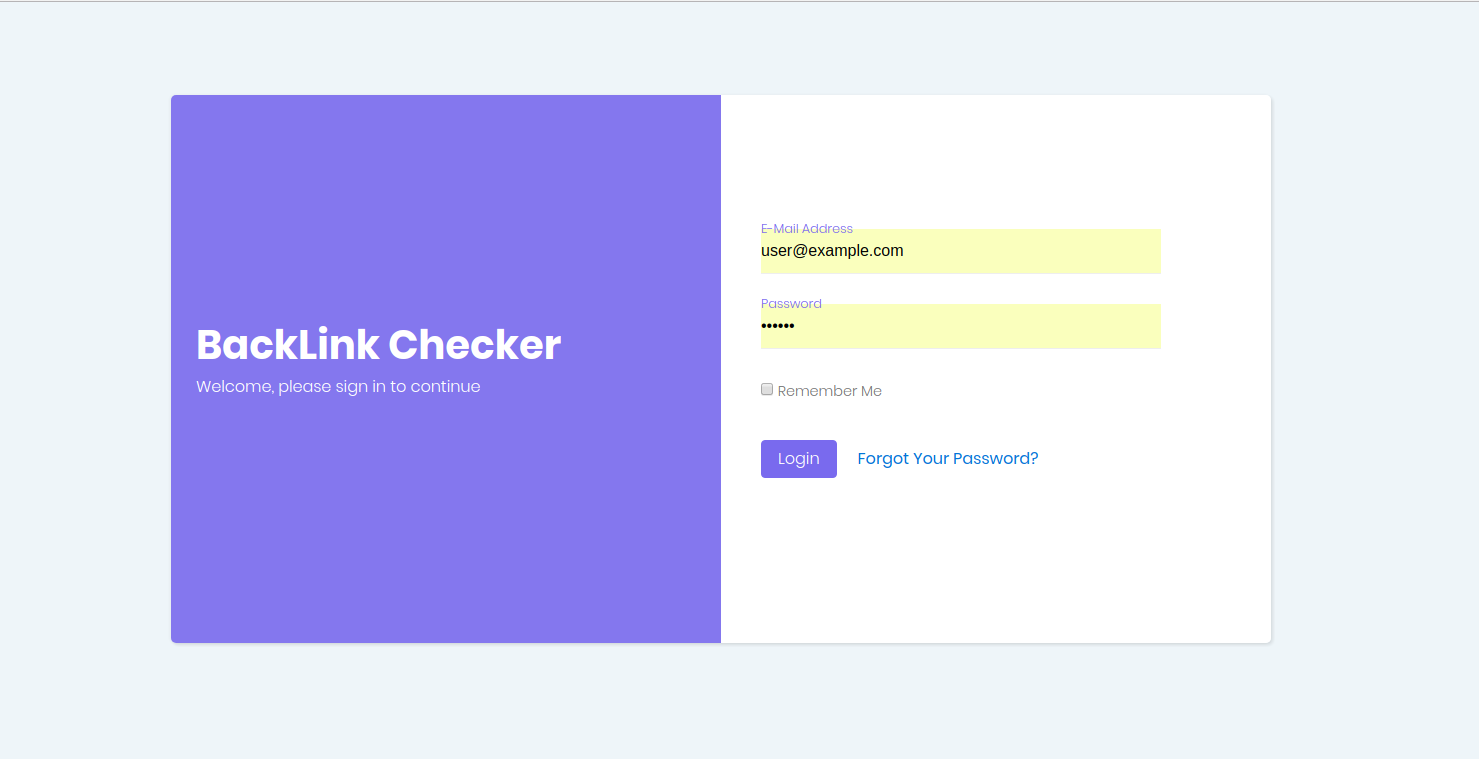
\includegraphics[width=\textwidth]{images/login_screenshot}
\end{figure*}

You need to put the user name (which is the email registered), then the password and click "Login" to get into the system, if the username or password is wrong you will not be able to login.

\textbf{Note:} When the system is a fresh install with the seed option set the default admin is admin@example.com with password set to ''secretadmin'', and the low privilege user is user@example.com with password set to ''secret'' always the passwords are without quotes.

\section{Users}
This section can only be accessed by the admin user, the regular user will not be able to use it. you access this section by clicking the left side bar link that states ''Users'', and you get presented a screen like the one below.
\begin{figure*}[ht!]
	\caption{Users screenshot}
	\label{img:login}
	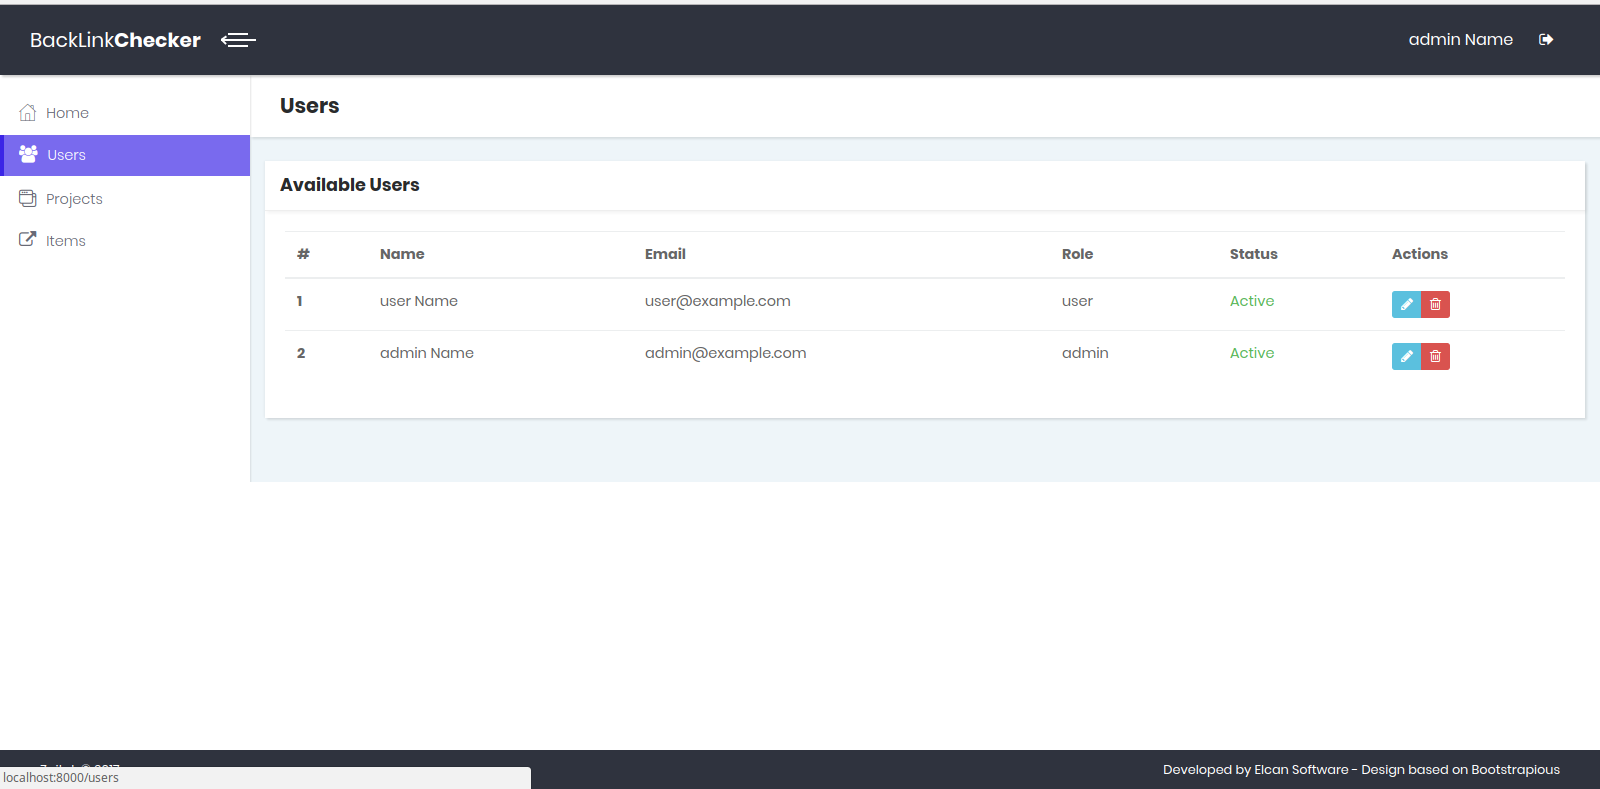
\includegraphics[width=\textwidth]{images/users_screenshot}
\end{figure*}

\section{Projects}

\section{Items}
